% \subsection{Smernice razvoja sistema}
% 
% Pri načrtovanju sistema za sestavljanje opisov tehnoloških postopkov smo se osredotočali predvsem na nasledje točke:
% \begin{itemize}
% 	% \item prekinitve dela, ki jih povzroči uporaba sistema morajo biti čim krajše,
% 	% \item uporabniški vmesnik odjemalca mora omogočati karseda učinkovito delo,
% 	\item uporabniški vmesniki sistema (mobilna aplikacija, glasovni pomočnik) morajo biti zamenjljivi,
% 	\item uporabljene podatke (fotografije, zapiske) se mora hraniti na enem mestu,
% 	\item sistem mora biti popolnoma funkcionalen brez glasovnega pomočnika.
% \end{itemize}
% 
% Sistem, ki smo ga implementirali v diplomski nalogi, služi kot primer kompleksnejšega sistema, katerega uporabnost bi radi izboljšali z uporabo glasovnega pomočnika.
% Z glasovnim pomočnikom smo poskusili implementirati dodajanje korakov v odprt projekt.

% \subsection{Zasnova aplikacije}

% Mobilna aplikacija služi kot osnovni način za interakcijo uporabnika s strežnikom.

% V diplomski nalogi preučujemo, ali je možno z vpeljavo glasovnega pomočnika v naš sistem izboljšati učinkovitost tega sistema.
% Da bodo rezultati dela čim bolj natančni, smo dali učinkovitosti mobilne aplikacije velik poudarek.
% Uporabniški vmesnik je bil zasnovan za čim hitrejše delo.
% To nam je v zagotovilo, da uporabniški vmesnik aplikacije ni ozko grlo pri pisanju opisov tehnoloških postopkov.

% \noindent Strežnik ima naslednje naloge:
% \begin{enumerate}
% 	\item komunikacija s podatkovno bazo,
% 	\item ponujanje vmesnika, preko katerega lahko odjemalci delajo s podatki v bazi (API),
% 	% \item komunikacija z odjemalcem (mobilno aplikacijo),
% 	\item komunikacija z glasovnim pomočnikom (Amazon Alexa).
% \end{enumerate}

\section{Implementacija mobilne aplikacije}

% Za osnovni uporabniški vmesnik našega sistema smo uporabili mobilno aplikacijo.
% Preko aplikacije se uporabnik lahko registrira in prijavi v sistem, dodaja, briše, odpira in izvaža svoje delavniške dnevnike.
% V delavniške dnevnike lahko dodaja korake, ki opisujejo delo, jih briše, spreminja vsebino ter ureja vrstni red.
% 
% Preko mobilne aplikacije lahko tudi zahteva in sprosti glasovnega pomočnika.
% Z mobilno napravo lahko zajema fotografije in jih v delavniške dnevnike dodal kot slikovno gradivo.
% 
% Mobilno aplikacijo smo uporabili kot primer odjemalca za naš strežnik (slika \ref{plan_server_client}).
% 
% Do strežnika dostopa preko API vmesnika.
% Zahtevki se prenašajo preko HTTP protokola.
% 
% Mobilno aplikacijo smo se odločili razviti s tehnologijo Xamarin.
% Razlogi za to so predvsem naše dobro poznavanje tehnologije in enostavna integracija z ostalimi tehnologijami iz .NET sklopa.

% Poskus prijave poteka tako, avtentikacijska storitev uporabniško ime in geslo zapiše v objekt razreda \texttt{LoginUserRequest}.
% Uporabniško ime in geslo se vneseta na prijavni strani.
% 
% \begin{Verbatim}[commandchars=+\[\]]
% LoginUserRequest {
%     string Email; 
%     string Password;
% }
% \end{Verbatim}
% 
% Nato se objekt \texttt{LoginUserRequest} pošlje na strežnik.
% Odjemalec ga pošlje na URL \enquote{\texttt{/identity/login}} preko POST metode.
% Strežnik ob uspešni avtentikaciji vrne objekt razreda \texttt{AuthSuccessResponse}.
% Iz tega objekta uporabnik prebere svoj avtorizacijski žeton.
% Ta žeton hrani avtentikacijska storitev.
% Komunikacijska storitev ta žeton doda v glavo nadaljnjih HTTP zahtevkov.
% 
% Če je avtentikacija neuspešna, strežnik vrne objekt razreda \texttt{AuthFailed-\\Response}, v katerem je podan opis napake.
% Ta opis napake se nato uporabniku izpiše na prijavni strani.
% 
% Stran za registracijo (slika \ref{app_register}) je podobna strani za prijavo, le, da ima dve vnosni polji za vpis gesla.
% Vrednost v obeh poljih za geslo mora biti enaka, da se lahko uporabnik registrira.
% 
% Registracijski zahtevek se pošlje na strežnik na URL \enquote{\texttt{/identity/regis-\\ter}}.
% Zahtevek je objekt razreda \texttt{RegisterUserRequest}.
% 
% \begin{Verbatim}[commandchars=+\[\]]
% RegisterUserRequest {
%     string Email; 
%     string Password;
% }
% \end{Verbatim}
% 
% \begin{figure}[H]
% \begin{center}
% 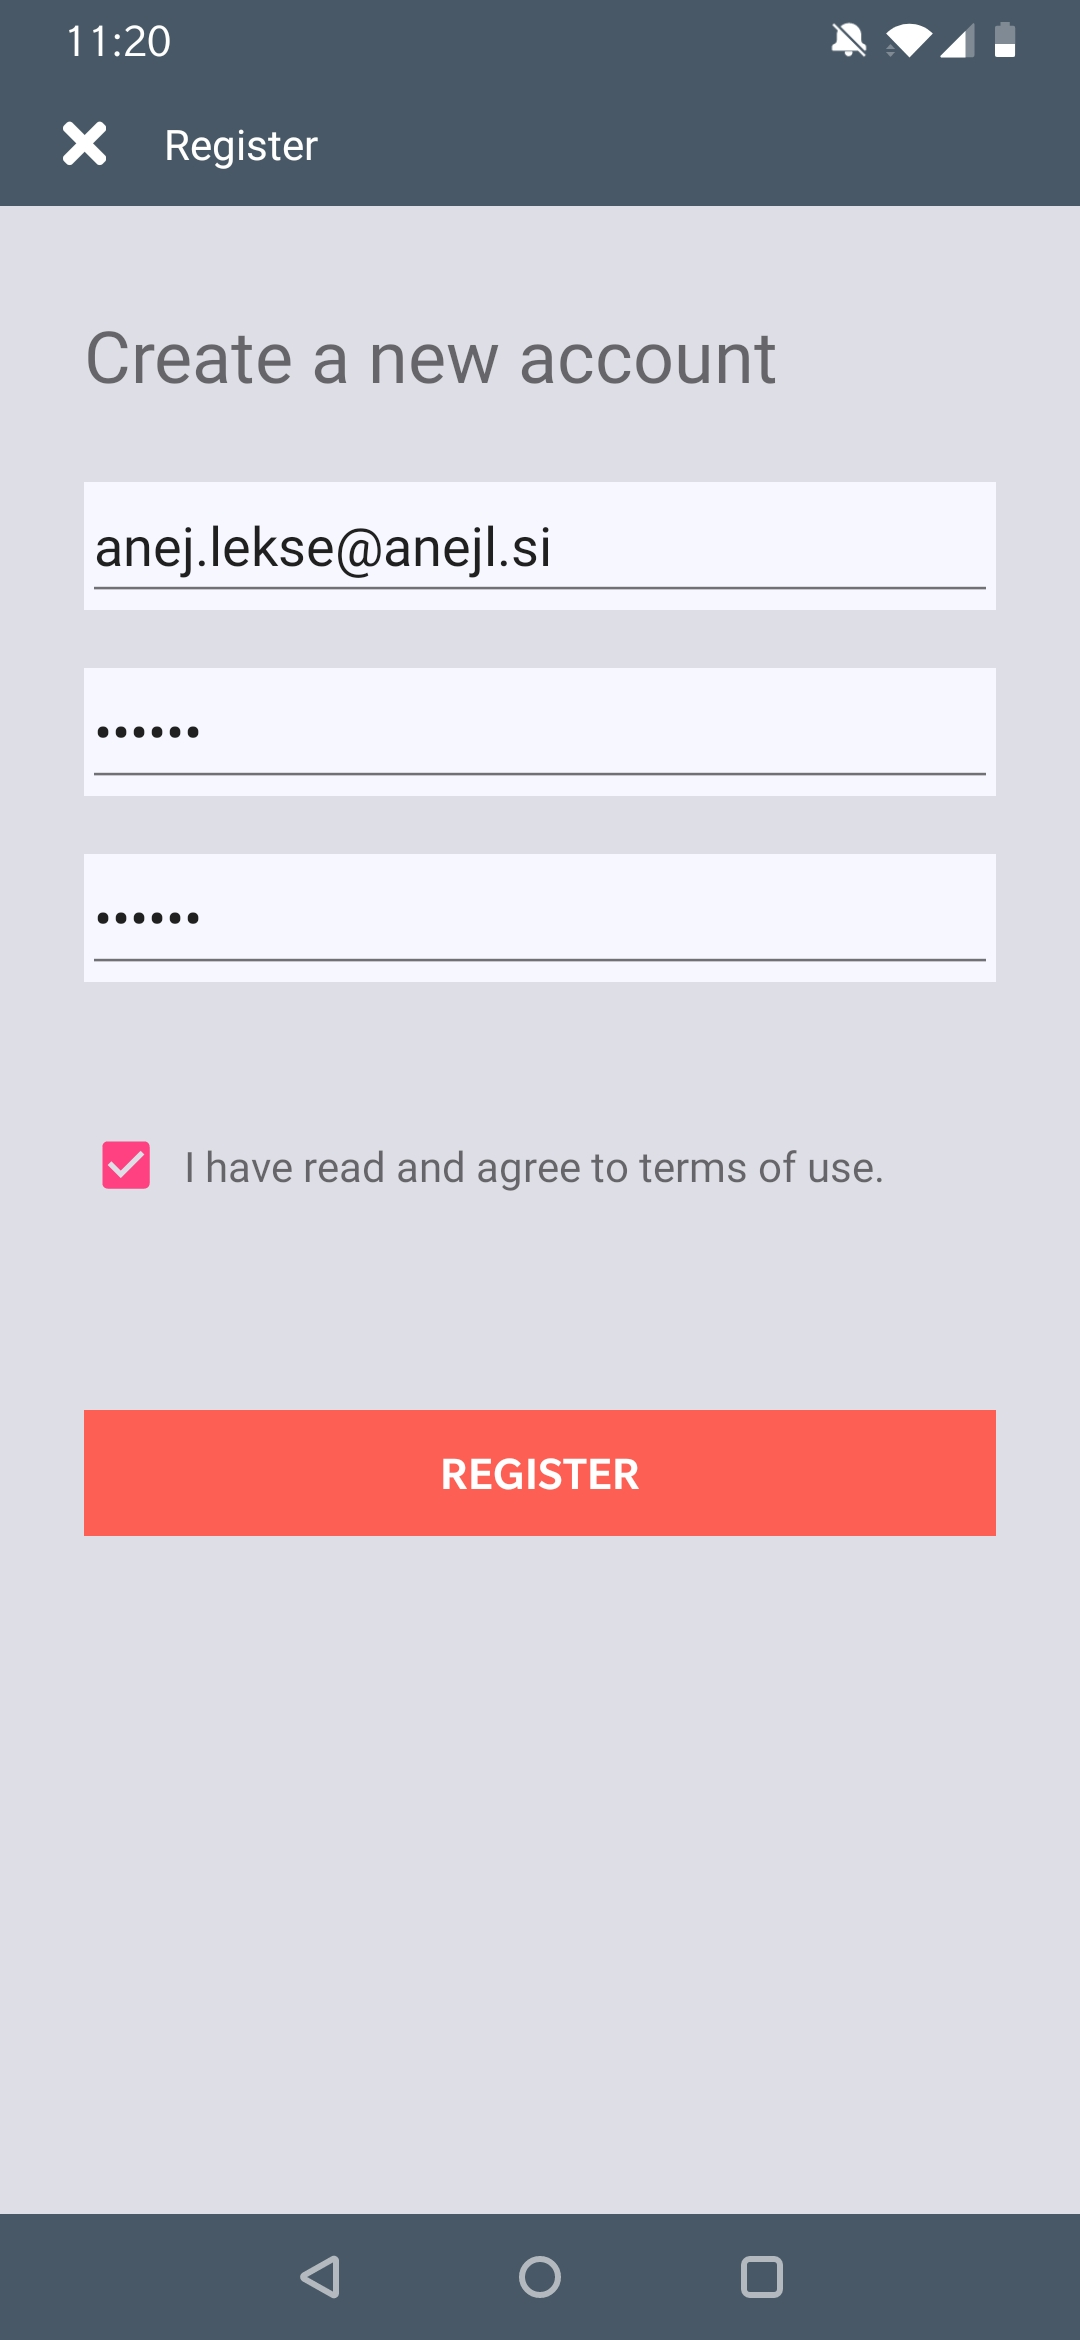
\includegraphics[width=4cm]{app_register}
% \end{center}
% 	\caption{Registracijska stran}
% \label{app_register}
% \end{figure}
% 
% \subsection{Ustvarjanje, brisanje in odpiranje projektov}


% \subsubsection{Ustvarjanje novega projekta}
% 
% Za ustvarjanje novega delavniškega dnevnika (slika \ref{app_newproject}), mora uporabnik odpreti stran za dodajanje projektov.
% Na tej strani mora vpisati naslov projekta (\texttt{Title}), kratek opis (\texttt{Description} in našteti možne nevarnosti pri delu \texttt{Dangers}.
% 
% Te tri vrednosti se zapišejo v objekt razreda \texttt{CreateProjectRequest}.
% \begin{Verbatim}[commandchars=+\[\]]
% CreateProjectRequest {
%     string Title;
%     string Description;
%     string Dangers;
% }
% \end{Verbatim}
% 
% Ta objekt nato storitev za komunikacijo s strežnikom pošlje preko metode POST na URL \enquote{\texttt{/projects/create}}.
% Strežnik v odgovor vrne objekt razreda \texttt{Project}, ki ga je zahtevek ustvaril.
% 
% Nov projekt se nato prikaže v seznamu vseh uporabnikovih projektov na strani \enquote{My Projects}, kjer ga lahko uporabnik odpre ali izbriše.
% 
% \begin{figure}[H]
% \begin{center}
% 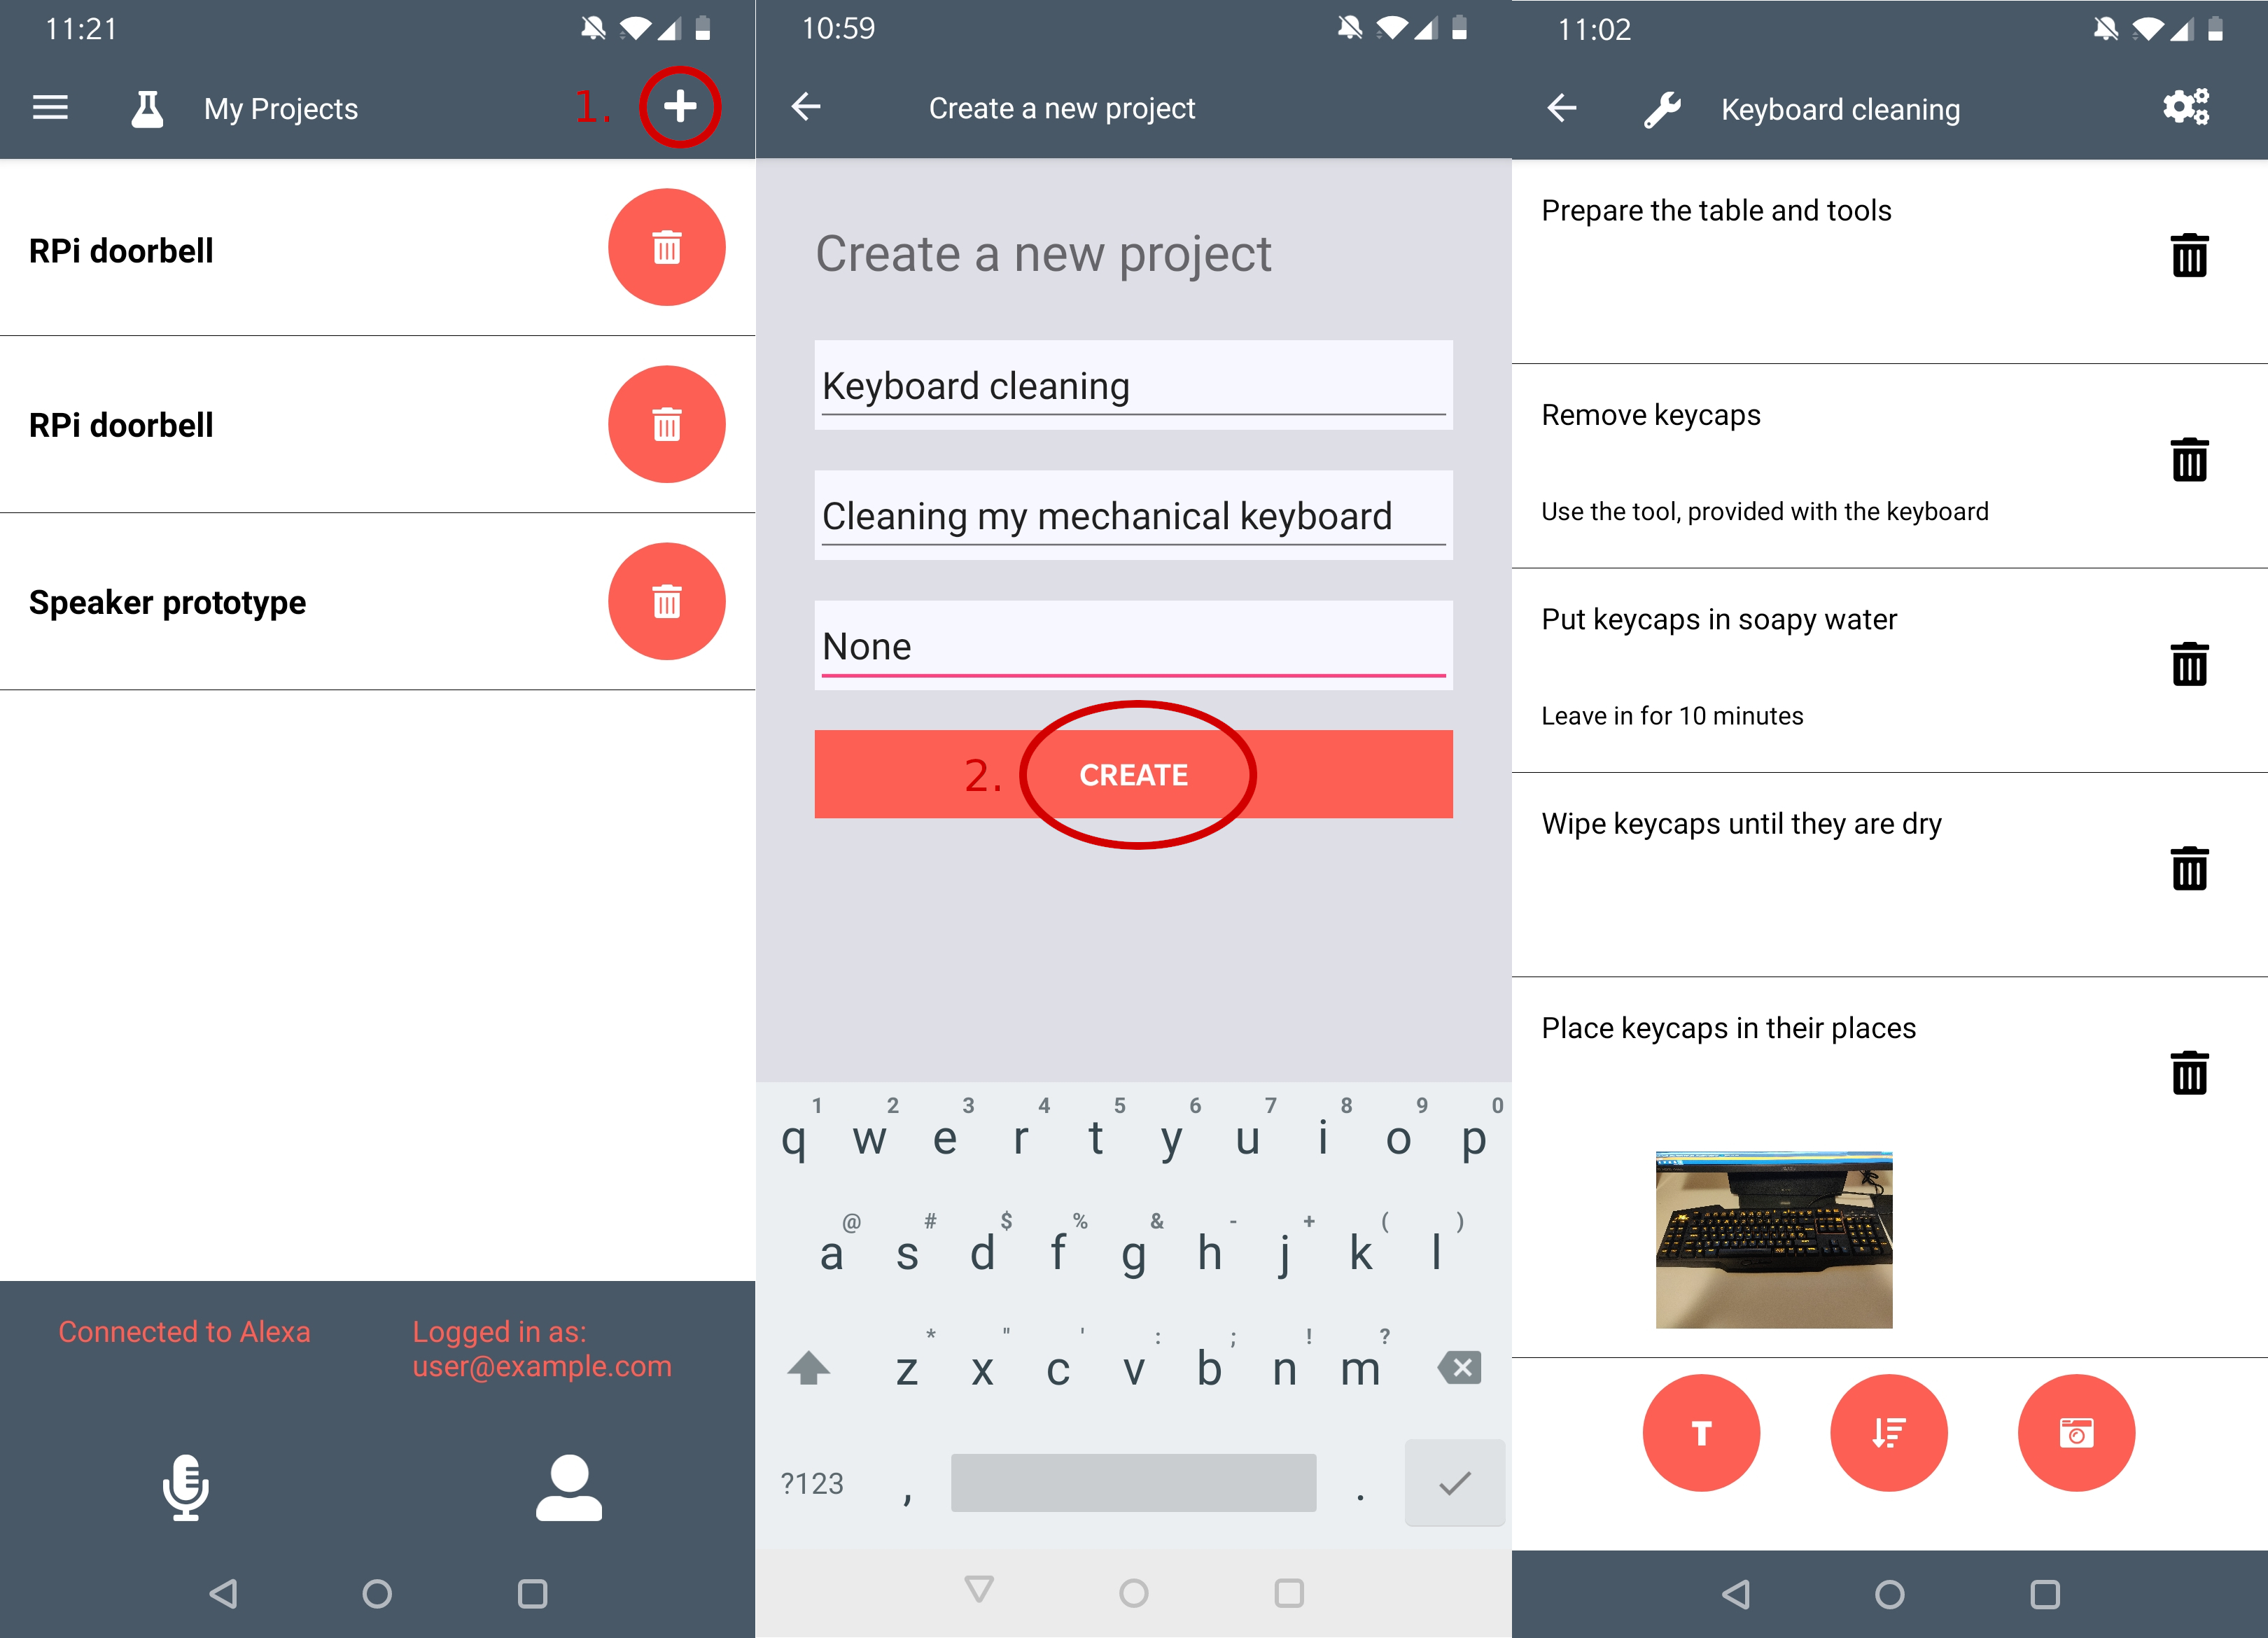
\includegraphics[width=13cm]{app_newproject}
% \end{center}
% 	\caption{Postopek ustvarjanja novega projekta po korakih.}
% \label{app_newproject}
% \end{figure}

% \subsubsection{Izbris projekta}
% 
% Da uporabnik izbriše delavniški dnevnik, mora na strani \enquote{My projects} ob željenem projektu pritisniti gumb z ikono smetnjaka.
% Pritisk na ta gumb sporoči storitvi za komunikacijo s strežnikom, naj pošlje avtoriziran DELETE zahtevek na URL \enquote{\texttt{/projects/\{id\}/delete}}.
% Strežnik ob uspešnem izbrisu projekta odjemalcu vrne kopijo izbrisanega projekta.

% \subsection{Dodajanje in brisanje zapiskov}
% 
% Ko ima uporabnik projekt odprt, lahko vanj dodaja korake, jih briše, ureja in jim spreminja vrstni red.
% Doda lahko tekstovni korak ali korak s fotografijo.
% 
% \begin{figure}[H]
% \begin{center}
% 	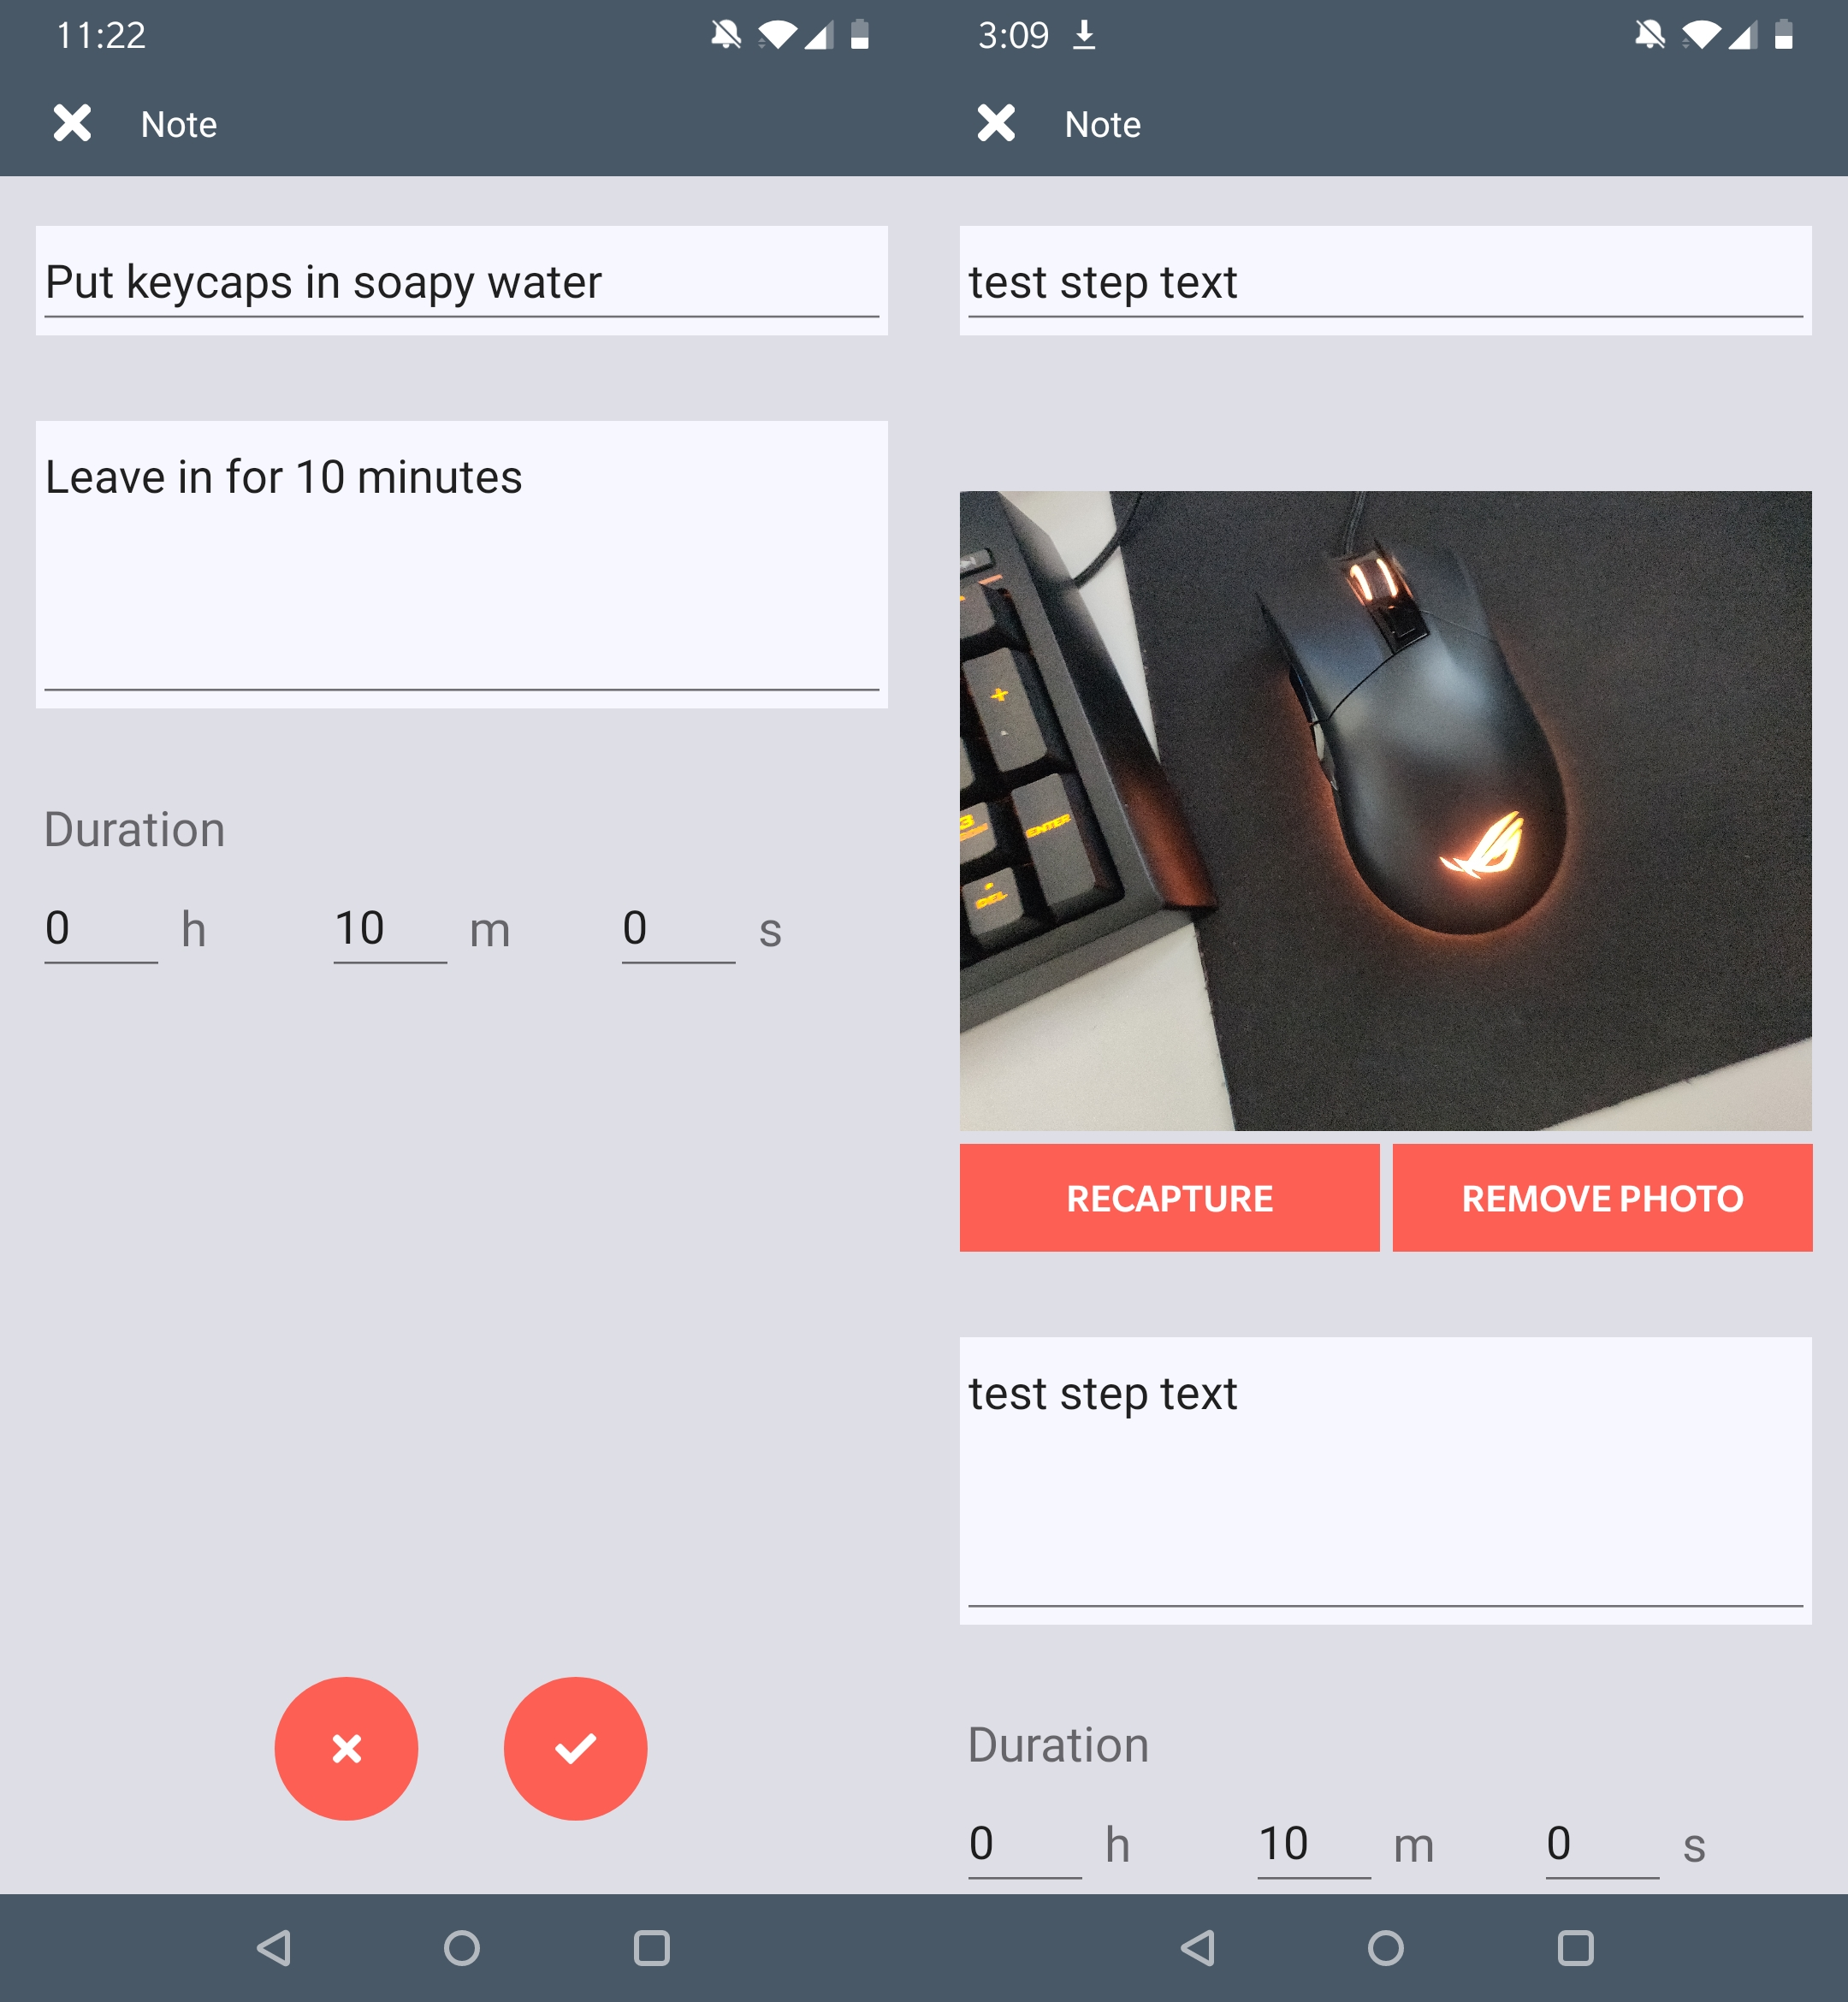
\includegraphics[width=9cm]{app_note_image}
% \end{center}
% 	\caption{Stran za dodajanje in urejanje korakov}
% \label{app_note}
% \end{figure}
% 
% Pri dodajanju besedilnega koraka mora uporabnik v vnosnem obrazcu (slika \ref{app_note}) podati naslov koraka (\texttt{Title}), opis koraka (\texttt{Text}) ter trajanje v urah, minutah in sekundah.
% Ti podatki se nato hranijo v objektu razreda \texttt{Note}.
% Ta objekt storitev za projekte vključi v objekt razreda \texttt{AddNoteRequest} in ga pošlje storitvi za komunikacijo s strežnikom.
% 
% \begin{Verbatim}[commandchars=+\[\]]
% AddNoteRequest { 
%     Note note; 
% }
% \end{Verbatim}
% 
% Storitev za komunikacijo s strežnikom pošlje ta objekt na strežnik.
% Pošlje ga na URL \enquote{\texttt{/projects/\{id\}/addnote}} preko metode POST.
% Polje \texttt{\{id\}} mora biti unikatni identifikator projekta, v katerega želimo korak vstaviti.
% Če je vstavljanje v projekt uspešno, strežnik odjemalcu pošlje v odgovor kopijo dodanega objekta \texttt{Note}.
% 
% Storitev za projekte nato ta korak doda svoji zbirki korakov.
% 
% Pri vstavljanju slikovnih korakov je postopek vstavljanja podoben.
% Uporabnik odpre stran za dodajanje slikovnega koraka in se zažene privzeta aplikacija za kamero.
% Fotografijo posname in ta se prikaže na strani z vnosnim obrazcem (slika \ref{app_note}).
% Slika se na mobilni napravi hrani v mapi \enquote{\texttt{Pictures/\{naslov projekta\}}}, v uporabnikovem domačem direktoriju.
% Uporabnik ima na vnosnem obrazcu možnost sliko ponovno posneti ali jo odstraniti.
% 
% Uporabnik mora v vnosnem obrazcu podati naslov koraka (\texttt{Title}), opis koraka (\texttt{Text}) ter trajanje v urah, minutah in sekundah.
% 
% Uporabnik mora nato pritisniti gumb za vstavljanje slikovnega koraka v projekt.
% Storitev za upravljanje s projektom fotografijo zakodira v znakovni niz po metodi Base64.
% Storitev za komunikacijo s strežnikom zakodirano fotografijo in novo ustvarjen objekt razreda \texttt{Note} vključi v objekt tipa \texttt{UploadImageRequest}.
% 
% \begin{Verbatim}[commandchars=+\[\]]
% UploadImageRequest {
%     Note note;
%     string ImageString; 
% }
% \end{Verbatim}
% 
% Novo nastali zahtevek \texttt{UploadImageRequest} se nato avtorizira z JWT avtorizacijskim žetonom in pošlje na URL \enquote{\texttt{/projects/\{id\}/addimage}}.
% Polje \texttt{\{id\}} mora biti unikatni identifikator projekta, v katerega želimo korak vstaviti.
% Če je vstavljanje v projekt uspešno, strežnik odjemalcu pošlje v odgovor kopijo pravkar vstavljenega objekta \texttt{Note}.

% \subsection{Izvoz projekta}
% 
% Uporabnik lahko projekt izvozi v človeško berljivo obliko na strežnik v dva različna formata: besedilno datoteko (.txt) in HTML dokument.
% 
% 
% Če želi uporabnik izvoziti projekt kot besedilno datoteko, storitev za komunikacijo s strežnikom pošlje POST zahtevek na URL \enquote{\texttt{/project/\{id\}/-\\export/text}}.
% Če želi uporabnik izvoziti projekt kot HTML dokument, storitev za komunikacijo s strežnikom pošlje POST zahtevek na URL \enquote{\texttt{/project-\\/\{id\}/export/html}}.


% \section{Testiranje sistema OpenReport}

% Sistem OpenReport smo po končani implementaciji testirali.
% Testiranje je bilo izvedeno tako, da smo s sistemom OpenReport sestavili delavniški dnevnik za čiščenje mehanske tipkovnice.
% 
% Najprej smo zagnali aplikacijo in se povezali na strežnik.
% Povezava na strežnik je bila uspešna.
% Če strežnik ni bil dosegljiv, se aplikacija ni ustavila.
% 
% Nato smo se prijavili z uporabniškim imenom \enquote{user@example.com} in geslom \enquote{string}.
% Ob napačno vpisanih podatkih je strežnik javil napako, ki se je izpisala pod prijavnim obrazcem.
% // TODO slika
% 
% Po uspešni prijavi smo na strani Dashboard zahtevali uporabo glasovnega asistenta.
% Nato smo odprli stran za dodajanje novega projekta (na sliki \ref{testproject} levo).
% Tam smo vpisali ime projekta, opis in možne nevarnosti (na sliki \ref{testproject} v sredini).
% 
% \begin{figure}[H]
% \begin{center}
% 	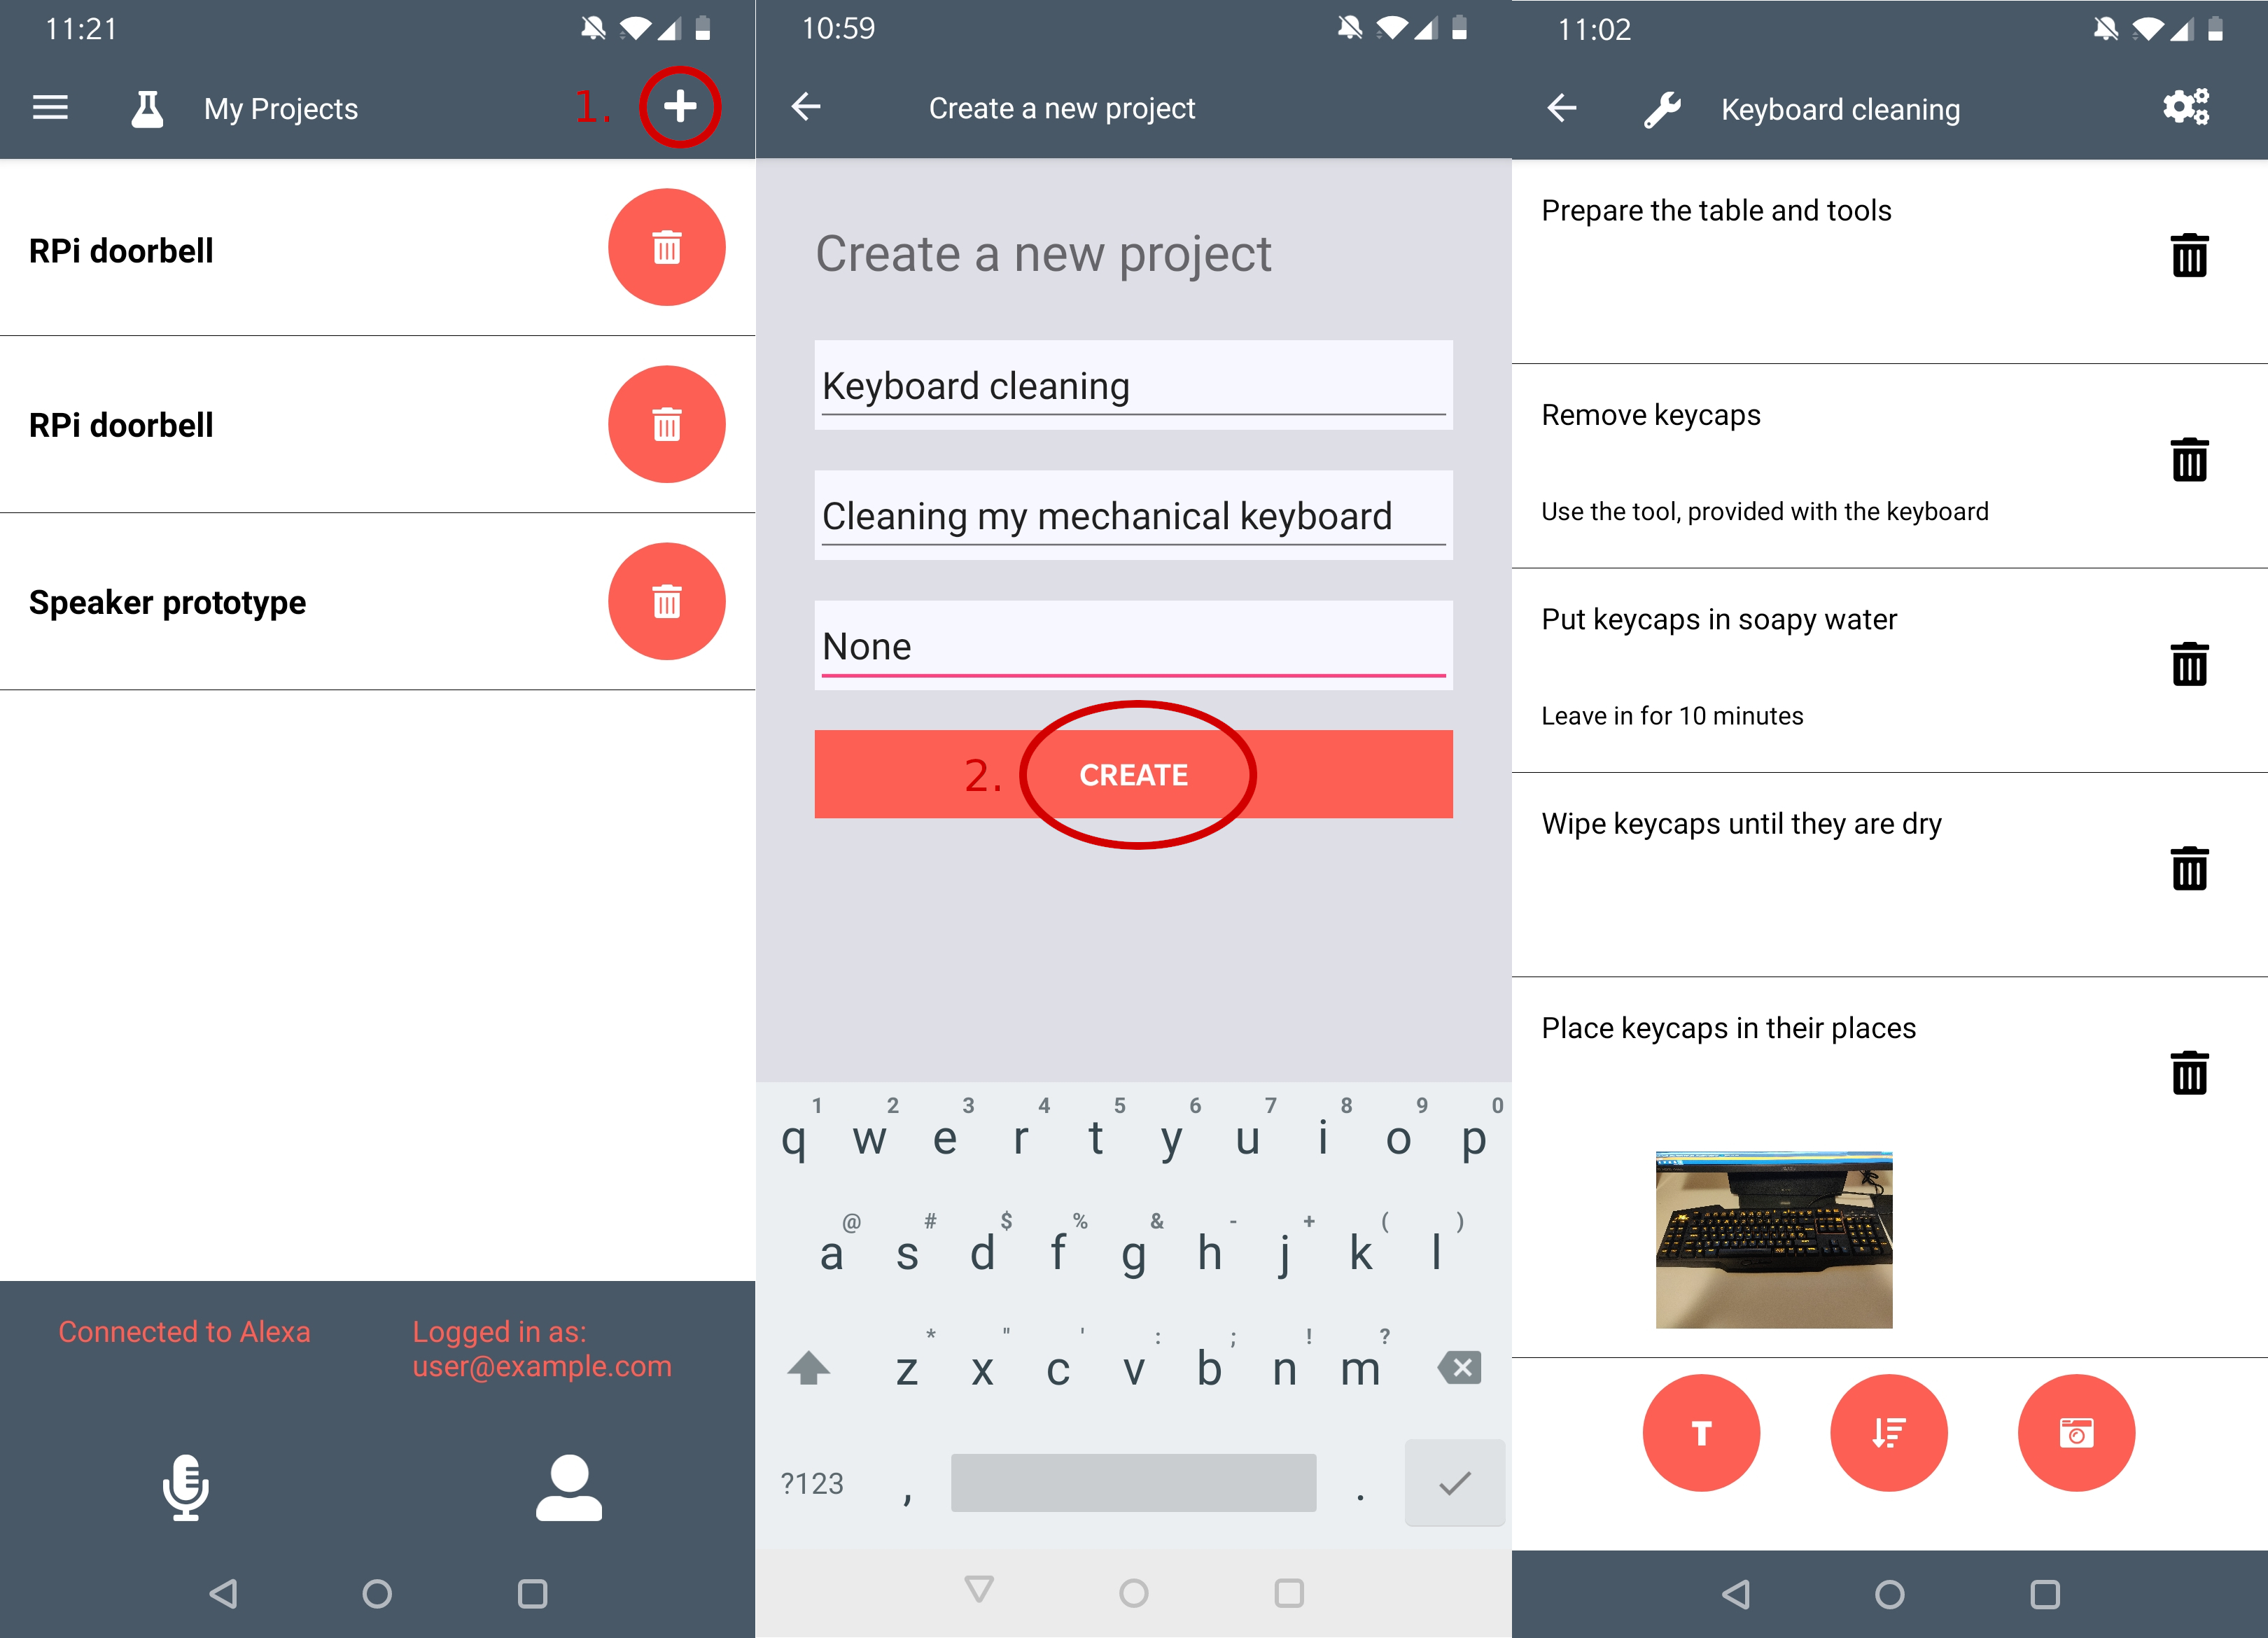
\includegraphics[width=13.5cm]{app_newproject}
% \end{center}
% 	\caption{Sestavljanje testnega delavniškega dnevnika za čiščenje tipkovnice.}
% \label{testproject}
% \end{figure}
% 
% Ko smo delavniški dnevnik ustvarili, smo začeli z dodajanjem korakov, ki so opisovali posamezne faze dela.
% 
% Testirali smo dodajanje korakov preko uporabniškega vmesnika aplikacije.
% Odprianje obrazca za dodajanje besedilnega koraka s pritiskom na gumb v aplikaciji ni povzročalo težav.
% Odprianje obrazca za dodajanje slikovnega koraka s pritiskom na gumb v aplikaciji ni povzročalo težav.
% 
% // TODO nadaljuj




% \subsection{Testne situacije}
% 
% Pripravili smo štiri testne situacije.
% 
% \begin{enumerate}
% 	\item Izdelava testnega opisa tehnološkega postopka \textbf{brez uporabe glasovnega pomočnika}
% 		\begin{enumerate}
% 			\item brez premora med koraki in
% 			\item z 90 sekundnim premorom med koraki.
% 		\end{enumerate}
% 	\item Izdelava testnega opisa tehnološkega postopka \textbf{z uporabo glasovnega pomočnika}
% 		\begin{enumerate}
% 			\item brez premora med koraki in
% 			\item z 90 sekundnim premorom med koraki.
% 		\end{enumerate}
% \end{enumerate}
% 
% Z 90 sekundnim premorom smo simulirali delo na izdelku.
% Med premorom vpišemo testne podatke v obrazec za dodajanje koraka.
% Po 90 sekundnem premoru korak vstavimo v poročilo.
% 
% \subsubsection{Testno poročilo}
% Testno poročilo mora vsebovati 4 tekstovne korake in enega slikovnega.
% Pri situacijah z uporabo Alexe, mora uporabnik obrazce za korake odpreti z glasovnim ukazom.
% 
% \subsection{Metoda testiranja in vpliv na hipotezo}
% 
% Testne situacije brez premorov so služile za preverjanje hitrosti dela.
% Hipotezo bomo potrdili, če bomo pisanje testnega poročila končali prej \emph{z uporabo Alexe} kot brez nje.
% 
% Če bo uporaba Alexe podaljšala čas pisanja, bomo hipotezo deloma ovrgli in prešli na drugo stopnjo testiranja.
% V drugi stopnji dodamo prejšnjemu postopku 90 sekundni premor med koraki.
% Ta premor simulira delo na izdelku.
% 
% Če bomo v tej situaciji poročilo z Alexo pisali enako hitro kot brez Alexe, hipoteza ostane delno ovržena.
% Če bo pisanje z Alexo počasnejše, kljub premorom, pa se bo hipotezo v celoti ovrglo.
% 
% \subsubsection{Testni koraki}
% 
% Testni koraki simulirajo delo na delovnem mestu, kjer se moramo za uporabo mobilnega telefona oddaljiti od delovnega mesta.
% 
% Testni korak za dodajanje besedilnega koraka je potekal tako:
% \begin{enumerate}
% 	\item premik do mobilnega telefona (3 metre),
% 	\item odpiranje obrazca za dodajanje besedilnega koraka,
% 	\item vpis besedila \enquote{Test step text},
% 	\item nastavitev trajanja na 10 minut,
% 	\item vstavljanje koraka,
% 	\item odmik od mobilnega telefona (3 metre).
% \end{enumerate}
% 
% \noindent Testni korak za dodajanje slikovnega koraka je potekal tako:
% \begin{enumerate}
% 	\item premik do mobilnega telefona (3 metre),
% 	\item odpiranje obrazca za dodajanje slikovnega koraka,
% 	\item zajem slike,
% 	\item vpis besedila \enquote{Test step text},
% 	\item nastavitev trajanja na 10 minut,
% 	\item vstavljanje koraka,
% 	\item odmik od mobilnega telefona (3 metre).
% \end{enumerate}
% 
% Pri situacijah z uporabo Amazon Alexe smo glasovne ukaze začeli izgovarjati, ko smo se začeli premikati proti mobilni napravi.
% 
% \subsection{Rezultati testiranja in ugotovitve}
% 
% \noindent\begin{tabular}{p{0.2\textwidth}|p{.3\textwidth}|p{.4\textwidth}}    
%   {\bf } & {\bf brez premorov}                             & {\bf z 90 sekundnimi premori} \\ \hline
%   {\bf brez Alexe} & 1 minuta 51 sekund & 7 minut 30 sekund \\
%   {\bf z Alexo} & 2 minuti 31 sekund & 7 minut 30 sekund \\
% \end{tabular}
% 
% \bigbreak
% \bigbreak
% % \noindent Iz tega sklepamo, da je hipoteza
% 
% Meritve časa pisanja poročil so pokazale, da je uporaba sistema OpenReport brez Amazon Alexe hitrejša v situacijah brez 90 sekundnih premorov.
% To našo hipotezo delno ovrže.
% V situacijah z 90 sekundnimi premori, je zapis korakov s pomočjo Amazon Alexe trajal enako dolgo kot brez nje.
% To našo hipotezo pusti delno ovrženo.
% 
% Testiranje zaključujemo z ugotovitvijo, da v situacijah brez premorov, Amazon Alexa dela ni pospešila.
% Hkrati pa smo ugotovili, da ga v testni situaciji s premori ni občutno ovirala.
% 
% Iz uporabniškega stališča prinese uporaba glasovnega pomočnika v proces interakcije z računalniškim sistemom novo dimenzijo.
% V našem primeru smo lahko zahtevo za odpiranje vnosnega obrazca v mobilni aplikaciji izvedli že na poti do naprave.

% Ta način bi pohitril delo, če bi lahko glasovni ukaz izgovorili in obdelali na poti do mobilne naprave.

% V naprednejših izvedbah računalniških sistemov z upravljanjem preko glasovnega pomočnika, bi na tak način lahko olajšali delo slabovidnim in gibalno omejenim posameznikom.
